\begin{prob}
    Run Bellman-Ford on the following graph using node $s$ as the source.
    Below each node $u$, write the shortest path length from $s$ to $u$.
    Mark the predecessor of $u$ by highlighting it or making a bold arrow.
    \begin{minted}[autogobble]{python}
        def bellman_ford(graph, weights, source):
            est={node:float('inf') for node in graph.nodes}
            est[source]=0
            predecessor={node: None for node in graph.nodes}
            for i in range(len(graph.nodes)-1):
                for(u, v) in graph.edges:
                    update(u, v, weights, est, predecessor)
            return est, predecessor
    \end{minted}

    \textbf{Edge ordering convention.}
    In each iteration (pass), perform \texttt{update(u, v)} exactly as listed below.
    Iteration pass uses this exact edge order:
    \[
        (s,a), (s,c), (c,a), (a,b), (b,c), (b,d), (d,c), (b,t), (d,t).
    \]
    Use this same edge order for every pass.

    \begin{center}
    	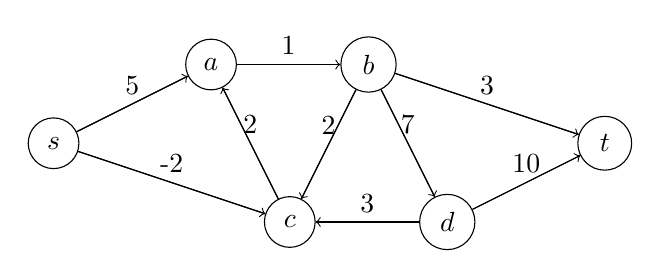
\begin{tikzpicture}
		    \tikzset{
   			vertex/.style={draw, circle, text width=8, align=center},
    			arc/.style={->}
		    }

   	        \draw node[vertex] (s) at (0,0) {$s$};
            \draw node[vertex] (a) at (2,1) {$a$};
            \draw node[vertex] (c) at (3,-1) {$c$};
			    \draw node[vertex] (d) at (5,-1) {$d$};
		        \draw node[vertex] (b) at (4,1) {$b$};
	              \draw node[vertex] (t) at (7,0) {$t$};
            \foreach \x/\y in {%
        	    s/a,s/c,c/a,a/b,b/c,b/d,d/c,b/t,d/t%
    	    }{
   		 	\draw (\x) edge[arc] (\y);
   	        }
            \draw[] (c) -- node[above] {2} (a);
            \draw[] (s) -- node[above] {5} (a);
            \draw[] (s) -- node[above] {-2} (c);
            \draw[] (a) -- node[above] {1} (b);
            \draw[] (b) -- node[above] {2} (c);
            \draw[] (b) -- node[above] {7} (d);
            \draw[] (d) -- node[above] {3} (c);
            \draw[] (b) -- node[above] {3} (t);
            \draw[] (d) -- node[above] {10} (t);
		    \end{tikzpicture}
    \end{center}
    \begin{responsebox}{3in}
    \end{responsebox}

    \begin{soln}
        Using the required edge order:
        \[
            (s,a), (s,c), (c,a), (a,b), (b,c), (b,d), (d,c), (b,t), (d,t).
        \]

        Pass 1 updates:
        \[
            a: \infty \to 5 \to 0,\;
            c: \infty \to -2,\;
            b: \infty \to 1,\;
            d: \infty \to 8,\;
            t: \infty \to 4.
        \]
        Pass 2: no values change, so the algorithm has converged.

        Final values:
        \begin{itemize}
            \item predecessor: $s\!:\!\texttt{None},\; a\!:\!c,\; b\!:\!a,\; c\!:\!s,\; d\!:\!b,\; t\!:\!b$
            \item est: $s\!:\!0,\; a\!:\!0,\; b\!:\!1,\; c\!:\!-2,\; d\!:\!8,\; t\!:\!4$
        \end{itemize}

        Notes:
        \begin{itemize}
            \item The edge ordering does not affect Bellman-Ford correctness.
            \item The edge ordering can affect how many passes are needed before convergence.
            \item If multiple shortest paths exist, different orderings can yield different predecessor trees.
        \end{itemize}
    \end{soln}
\end{prob}
